
%(BEGIN_QUESTION)
% Copyright 2006, Tony R. Kuphaldt, released under the Creative Commons Attribution License (v 1.0)
% This means you may do almost anything with this work of mine, so long as you give me proper credit

Tegn utgangen for denne regulatoren med bare P-ledd, gitt gain ($K_p$) lik 2.0, bias lik 50\%, og direktevirkende reguleringsvirkning:

$$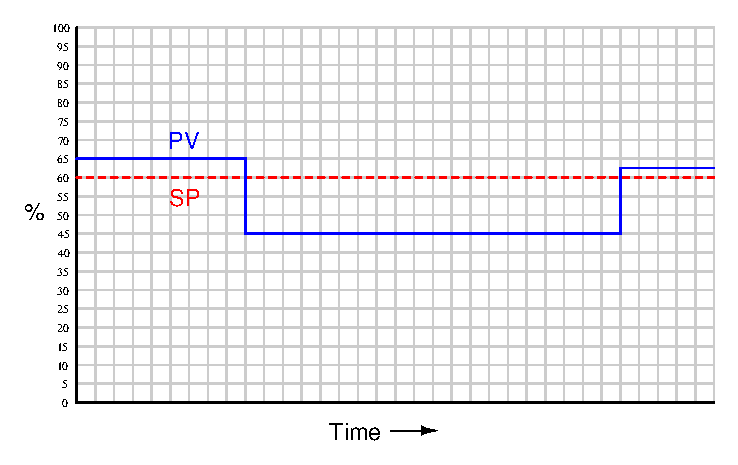
\includegraphics[width=15.5cm]{i01468x01.eps}$$

\vskip 20pt \vbox{\hrule \hbox{\strut \vrule{} {\bf Forslag til sokratisk diskusjon} \vrule} \hrule}

\begin{itemize}
\item{} Forklar hvorfor denne trendgrafen for PV er urealistisk for en virkelig prosess, men likevel nyttig for å lære hvordan en regulator med bare P-ledd er ment å reagere på endringer i PV.
\item{} Hvordan tror du PV {\it faktisk} ville reagert i en virkelig prosess under forholdene som vises (eller antydes) i trenden? Skisser en mer realistisk respons for en riktig innstilt regulator med bare P-ledd i automatisk modus.
\end{itemize}

\underbar{file i01468}
%(END_QUESTION)





%(BEGIN_ANSWER)

$$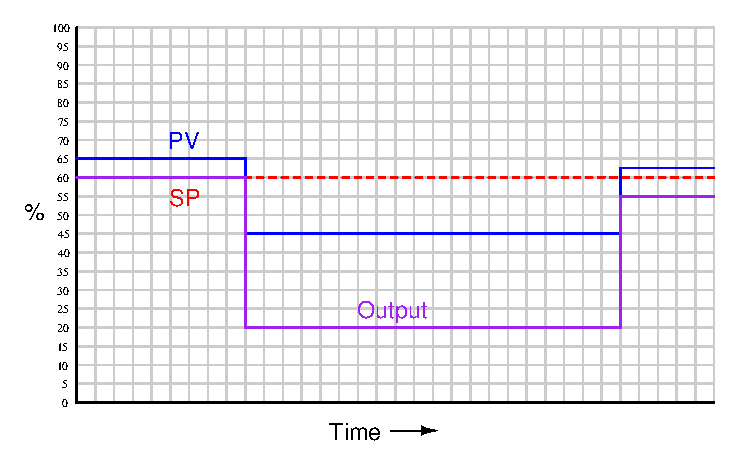
\includegraphics[width=15.5cm]{i01468x02.eps}$$

%(END_ANSWER)





%(BEGIN_NOTES)


\vfil \eject

\noindent
{\bf Oppsummeringsquiz:}

Regulatoren som lager utgangen i denne trenden er konfigurert for:

$$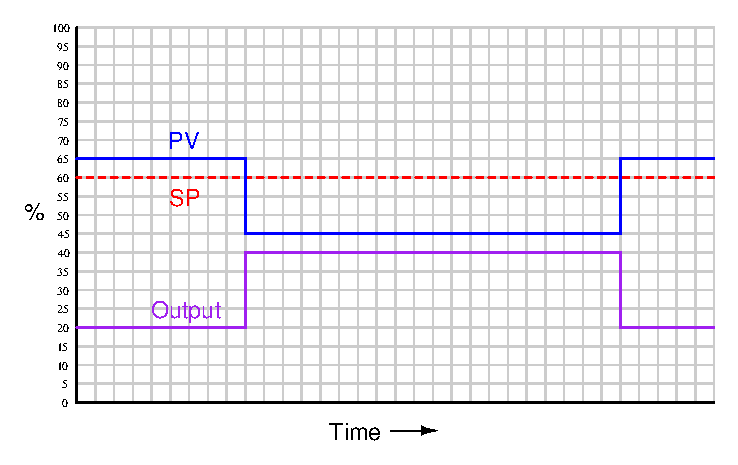
\includegraphics[width=15.5cm]{i01468x03.eps}$$

\begin{itemize}
\item{} Direkte reguleringsvirkning
\vskip 5pt 
\item{} En proporsjonalbåndverdi på 100\%
\vskip 5pt 
\item{} En gain-verdi på 1.5
\vskip 5pt 
\item{} En proporsjonalbåndverdi på 15\%
\vskip 5pt 
\item{} En gain-verdi på 0.5
\vskip 5pt 
\item{} En proporsjonalbåndverdi på 400\%
\end{itemize}



%INDEX% Control, proportional: graphing controller response

%(END_NOTES)

